\documentclass[t,usenames,dvipsnames]{beamer}
\usetheme{Copenhagen}
\setbeamertemplate{headline}{} % remove toc from headers
\beamertemplatenavigationsymbolsempty

\usepackage{amsmath, xcolor, tikz, pgfplots, array}

\pgfplotsset{compat = newest}
\usetikzlibrary{arrows.meta, calc, decorations.pathreplacing}
\pgfplotsset{every axis/.append style = {axis lines = middle}}
\pgfplotsset{every tick label/.append style={font=\scriptsize}}
\everymath{\displaystyle}

\title{Polynomial and Rational Inequalities}
\author{}
\date{}

\AtBeginSection[]
{
  \begin{frame}
    \frametitle{Objectives}
    \tableofcontents[currentsection]
  \end{frame}
}

\begin{document}

\begin{frame}
    \maketitle
\end{frame}

\section{Solve polynomial inequalities}

\begin{frame}{Polynomial Inequalities}
    When solving polynomial inequalities, first \alert{find the zeros} of the polynomial (may have to get = to 0 first). \newline\\ \pause
    
    Then, set up a number line and \alert{use test values}.
\end{frame}

\begin{frame}{Example 1}
Solve $8x^3 - 2x^2 > 41x + 10$. Write your answer in interval notation.
\begin{align*}
    \onslide<2->{8x^3 - 2x^2 &> 41x + 10}\\[6pt]
    \onslide<3->{8x^3 - 2x^2 - 41x - 10 &> 0}
\end{align*}
\begin{center}
    \onslide<4->{Zeros at $x = -2, \, -\frac{1}{4}, \, \frac{5}{2}$ \\[15pt]}
\onslide<5->{
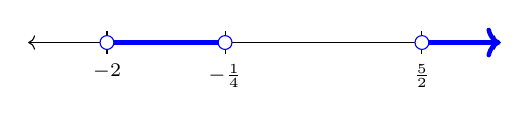
\begin{tikzpicture}
\draw[<->] (-3,0) -- (3,0);
\draw (-2,0.15) -- (-2,-0.15) node [below] {\scriptsize $-2$};
\draw (-0.5,0.15) -- (-0.5,-0.15) node [below] {\scriptsize $-\tfrac{1}{4}$};
\draw (2,0.15) -- (2,-0.15) node [below] {\scriptsize $\tfrac{5}{2}$};
\onslide<7->{\draw [color=blue, ultra thick, shorten <= 2.5pt, shorten >= 2.5pt] (-2,0) -- (-0.5,0);}
\onslide<7->{\draw [->,color=blue, ultra thick, shorten <= 2.5pt] (2,0) -- (3,0);}
\onslide<6->{\draw [color=blue,fill=white] (-2,0) circle [radius = 2.5pt];}
\onslide<6->{\draw [color=blue,fill=white] (-0.5,0) circle [radius = 2.5pt];}
\onslide<6->{\draw [color=blue,fill=white] (2,0) circle [radius = 2.5pt];}
\end{tikzpicture}}
\end{center}
\end{frame}

\begin{frame}[c]{Example 1}
\[8x^3 - 2x^2 - 41x - 10 > 0 \]
\begin{center}
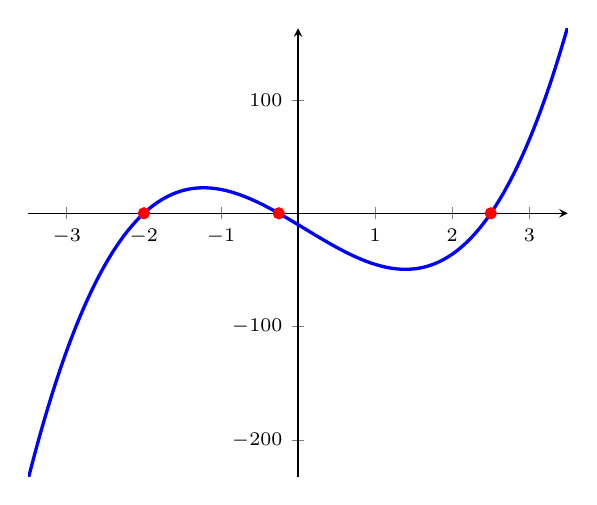
\begin{tikzpicture}
\begin{axis}[
xmin = -3.5, xmax = 3.5,
]
\addplot [color=blue, very thick, samples = 200, smooth] {8*x^3-2*x^2-41*x-10};
\addplot [color=red, mark = *, only marks] coordinates {(-2,0) (-0.25,0) (2.5,0)};
\end{axis}
\end{tikzpicture}
\end{center}
\end{frame}

\section{Solve rational inequalities}

\begin{frame}{Rational Inequalities}
When solving rational inequalities, your \alert{critical values} will be where the {\color{blue}\textbf{denominator = 0}} and the {\color{blue}\textbf{solution to the inequality as an equation}}.  \newline\\  \pause

\emph{Note:} The critical values of the {\color{blue}\textbf{denominator}} will \underline{always} be open circles on the number line.
\end{frame}

\begin{frame}{Example 2}
Solve each. Write your answers using interval notation. \newline\\
(a) \quad $\frac{3x+9}{2x-5} \leq 0$
\begin{align*}
    \onslide<2->{2x-5&=0 & \onslide<4->{3x+9&=0}} \\
    \onslide<3->{x&=\frac{5}{2} & \onslide<5->{x&=-3}} \\
\end{align*}
\begin{center}
\onslide<6->{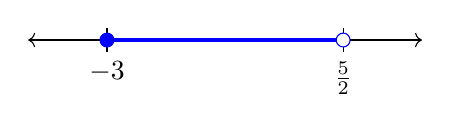
\begin{tikzpicture}
\draw[<->] (-2.5,0) -- (2.5,0);
\draw (-1.5,0.15) -- (-1.5,-0.15) node [below] {$-3$};
\draw (1.5,0.15) -- (1.5,-0.15) node [below] {$\tfrac{5}{2}$};
\onslide<7->{\draw[color=blue, fill=blue] (-1.5,0) circle [radius=2.5pt];}
\onslide<8->{\draw[color=blue, fill=white] (1.5,0) circle [radius=2.5pt];}
\onslide<9->{\draw[color=blue, ultra thick, shorten >= 2.5pt] (-1.5,0) -- (1.5,0);}
\end{tikzpicture}}
\end{center}
\onslide<7->{\[\left[-3, \frac{5}{2}\right) \]}
\end{frame}

\begin{frame}{Example 2}
(b) \quad $\frac{4-x}{x+1} > 2$
\begin{align*}
    \onslide<2->{x+1 &=0    &  \onslide<4->{\frac{4-x}{x+1} &= \frac{2}{1}} } \\[8pt]
    \onslide<3->{x &= -1    &  \onslide<5->{2(x+1) &= 4-x} } \\[8pt]
    \onslide<6->{&  &   2x+2 &= 4-x} \\[8pt]
    \onslide<7->{&  &   3x &= 2} \\[8pt]
    \onslide<8->{&  &   x &= \frac{2}{3}}
\end{align*}
\end{frame}

\begin{frame}[c]{Example 2 \quad $\frac{4-x}{x+1} > 2$}
\begin{center}
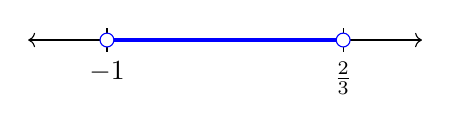
\begin{tikzpicture}
\draw[<->] (-2.5,0) -- (2.5,0);
\draw (-1.5,0.15) -- (-1.5,-0.15) node [below] {$-1$};
\draw (1.5,0.15) -- (1.5,-0.15) node [below] {$\frac{2}{3}$};
\onslide<2->{\draw[color=blue, fill=white] (-1.5,0) circle [radius=2.5pt];}
\onslide<2->{\draw[color=blue, fill=white] (1.5,0) circle [radius=2.5pt];}
\onslide<3->{\draw[color=blue, ultra thick, shorten <= 2.5pt, shorten >= 2.5pt] (-1.5,0) -- (1.5,0);}
\end{tikzpicture}
\end{center}
\onslide<4->{\[\left(-1, \frac{2}{3}\right)\]}
\end{frame}

\begin{frame}{Example 2}
\[\frac{4-x}{x+1} > 2\]
\begin{center}
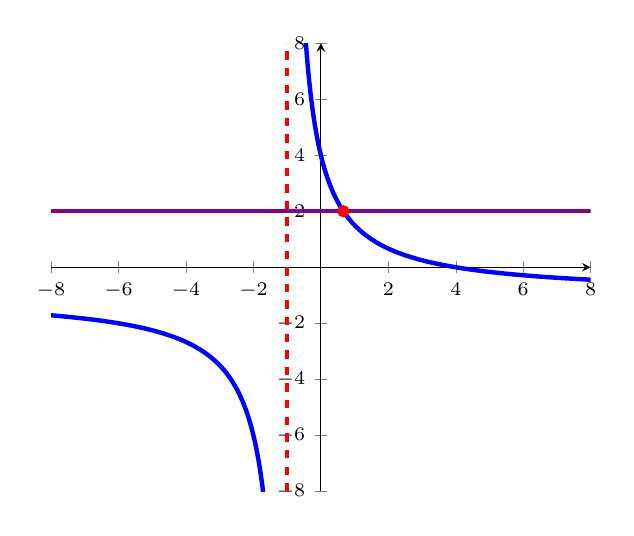
\begin{tikzpicture}
\begin{axis}[
xmin = -8, xmax = 8,
ymin = -8, ymax = 8,
xtick = {-8,-6,...,8},
ytick = {-8,-6,...,8}
]
\addplot[color=blue, ultra thick, samples=200, smooth, domain=-8:-1.05] {(4-x)/(x+1)};
\addplot[color=blue, ultra thick, samples=200, smooth, domain=-0.95:8] {(4-x)/(x+1)};
\addplot[color=violet, ultra thick, domain=-8:8] {2};
\draw[color=red, ultra thick, dashed] (axis cs: -1,-8) -- (axis cs: -1,8);
\addplot[color=red, mark = *] coordinates {(0.667,2)};
\end{axis}
\end{tikzpicture}
\end{center}
\end{frame}

\begin{frame}{Example 2}
(c) \quad $\frac{x^2-3x-4}{x^2-4x+3} \geq 0$
\begin{align*}
    \onslide<2->{x^2-3x-4&=0 & x^2-4x+3&=0} \\[6pt]
    \onslide<3->{(x-4)(x+1)&=0 & (x-3)(x-1)&=0} 
\end{align*}
\begin{align*}
    \onslide<4->{x-4&=0 & x+1&=0 & x-3&=0 & x-1&=0} \\[6pt]
    \onslide<5->{x&=4 & x&=-1 & x&=3 & x&=1} \\[-8pt]
\end{align*}
\begin{center}
\onslide<6->{
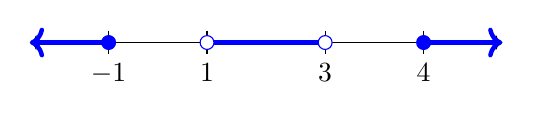
\begin{tikzpicture}
\draw[<->] (-3,0) -- (3,0);
\draw (-2,0.15) -- (-2,-0.15) node [below] {$-1$};
\draw (-0.75,0.15) -- (-0.75,-0.15) node [below] {$1$};
\draw (0.75,0.15) -- (0.75,-0.15) node [below] {$3$};
\draw (2,0.15) -- (2,-0.15) node [below] {$4$};
\onslide<7->{\draw[color=blue, fill=blue] (-2,0) circle [radius=2.5pt];}
\onslide<7->{\draw[color=blue, fill=blue] (2,0) circle [radius=2.5pt];}
\onslide<8->{\draw[color=blue, fill=white] (-0.75,0) circle [radius=2.5pt];}
\onslide<8->{\draw[color=blue, fill=white] (0.75,0) circle [radius=2.5pt];}
\onslide<9->{\draw[color=blue, ultra thick, ->] (-2,0) -- (-3,0);}
\onslide<9->{\draw[color=blue, ultra thick, shorten <= 2.5pt, shorten >= 2.5pt] (-0.75,0) -- (0.75,0);}
\onslide<9->{\draw[color=blue, ultra thick, ->] (2,0) -- (3,0);}
\end{tikzpicture}
}
\end{center}
\onslide<10->{\[(-\infty, -1] \cup (1,3) \cup [4, \infty)\]}
\end{frame}

\begin{frame}{Example 2}
\[\frac{x^2-3x-4}{x^2-4x+3} \geq 0\]
\begin{center}
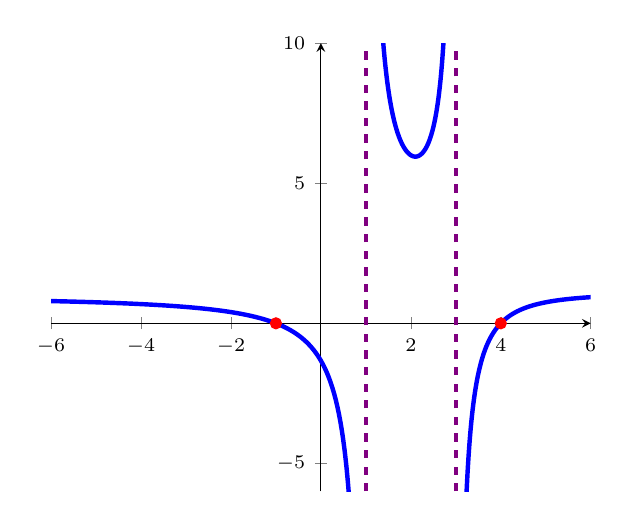
\begin{tikzpicture}
\begin{axis}[
xmin = -6, xmax = 6,
ymin = -6, ymax = 10
]
\addplot[color=blue, ultra thick, samples=200, smooth, domain=-6:0.95] {(x^2-3*x-4)/(x^2-4*x+3)};
\addplot[color=blue, ultra thick, samples=200, smooth, domain=1.05:2.95] {(x^2-3*x-4)/(x^2-4*x+3)};
\addplot[color=blue, ultra thick, samples=200, smooth, domain=3.05:6] {(x^2-3*x-4)/(x^2-4*x+3)};
\addplot[color=red, mark=*, only marks] coordinates {(-1,0) (4,0)};
\draw [color=violet, dashed, ultra thick] (axis cs: 1,-6) -- (axis cs: 1,10);
\draw [color=violet, dashed, ultra thick] (axis cs: 3,-6) -- (axis cs: 3,10);
\end{axis}
\end{tikzpicture}
\end{center}
\end{frame}

\begin{frame}{Example 2}
(d) \quad $\frac{x+2}{x-3} < 2x-2$
\begin{align*}
    \onslide<2->{x-3 &= 0 & \onslide<4->{\frac{x+2}{x-3} &= \frac{2x-2}{1}}} \\[8pt]
    \onslide<3->{x &= 3 & \onslide<5->{(2x-2)(x-3) &= x+2}} \\[8pt]
    \onslide<6->{& & 2x^2-8x+6 &= x+2} \\[8pt]
    \onslide<7->{& & 2x^2 - 9x + 4 &= 0} \\[8pt]
    % \onslide<4->{\frac{x+2}{x-3} &= \frac{2x^2-8x+6}{x-3}} \\[8pt]
    % \onslide<5->{x+2 &= 2x^2 - 8x + 6} \\[6pt]
    % \onslide<6->{2x^2 - 9x + 4 &= 0} \\[6pt]
    \onslide<8->{& & x &= \frac{1}{2}, \, 4}
\end{align*}
\end{frame}

\begin{frame}{Example 2 \quad $\tfrac{x+2}{x-3} < 2x-2$}
Critical values: $x = \frac{1}{2}, \, {\color{red}3}, \, 4$ \\[1cm]
\begin{center}
\onslide<2->{
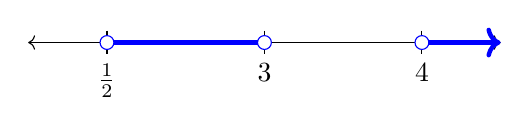
\begin{tikzpicture}
\draw[<->] (-3,0) -- (3,0);
\draw (-2,0.15) -- (-2,-0.15) node [below] {$\tfrac{1}{2}$};
\draw (0,0.15) -- (0,-0.15) node [below] {$3$};
\draw (2,0.15) -- (2,-0.15) node [below] {$4$};
\onslide<3->{\draw[color=blue, fill=white] (-2,0) circle [radius=2.5pt];}
\onslide<3->{\draw[color=blue, fill=white] (0,0) circle [radius=2.5pt];}
\onslide<3->{\draw[color=blue, fill=white] (2,0) circle [radius=2.5pt];}
\onslide<4->{\draw[color=blue, ultra thick, shorten <= 2.5pt, shorten >= 2.5pt] (-2,0) -- (0,0);}
\onslide<4->{\draw[color=blue, ultra thick, shorten <= 2.5pt, ->] (2,0) -- (3,0);}
\end{tikzpicture}}
\end{center}    \vspace{0.5cm}
\onslide<5->{\[\left(\frac{1}{2}, 3\right) \cup (4, \infty)\]}
\end{frame}

\end{document}
